\documentclass{beamer}
\usepackage{xcolor}
\usepackage{graphicx}
\usepackage{tikz}
\usetikzlibrary{arrows, positioning, decorations.pathmorphing, patterns}
\usetheme{metropolis}

% title, names, ...
\date{\today}
\author{Lukas Westhofen \and Christoph Welzel}
\institute{ComSys, RWTH Aachen}
\title{Submarine \hspace{4.2cm}\parbox{4cm}{\resizebox{4cm}{!}{\includegraphics{pic/logo}}}}
\subtitle{Team Voltidioten}

% metropolis theme configuration
\definecolor{CorporateRose}{HTML}{F6ABC0}
\definecolor{DarkKhaki}{HTML}{BDB76B}
\definecolor{NavyBlue}{HTML}{000080}

\setbeamercolor{normal text}{bg=white, fg=black}
\setbeamercolor{progress bar}{bg=CorporateRose, fg=CorporateRose}
\setbeamercolor{title separator}{fg=CorporateRose, bg=CorporateRose}
\setbeamercolor{frametitle}{parent=structure, bg=CorporateRose}
\metroset{numbering=fraction}

\begin{document}

	\maketitle

	\section{Idea}
	\begin{frame}{Sketch: Concept}
		\begin{center}
			\resizebox{0.7\textwidth}{!}{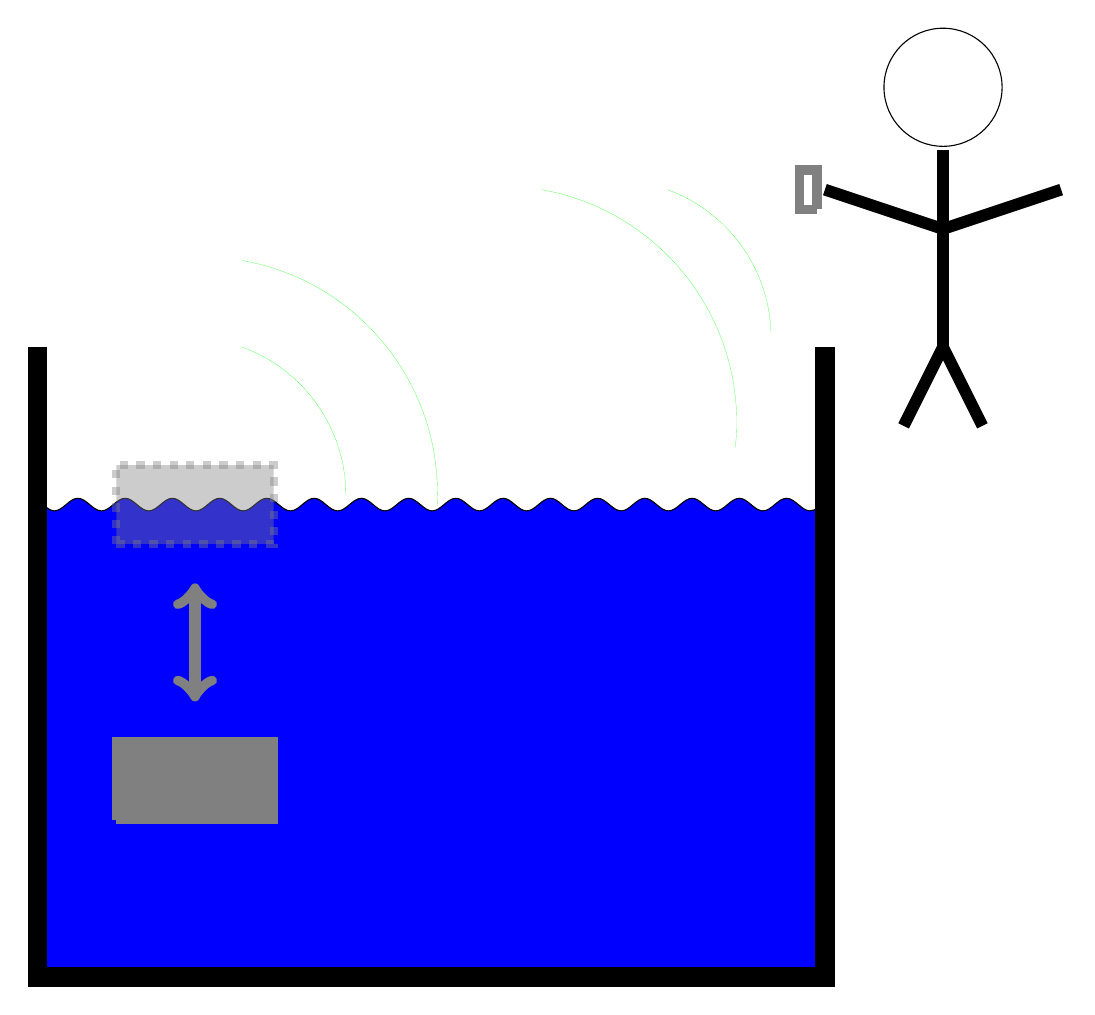
\begin{tikzpicture}
	\draw[
		decoration={
			snake,
			amplitude=0.8mm,
			segment length=6mm
		},
		fill=blue
	] decorate {(10,6) -- (0,6)} -- (0,0) -- (10,0) -- (10,6);
	\draw[
		line width=0.25cm
	] (10,8) -- (10,0) -- (0,0) -- (0,8);
	\draw[
		color=gray,
		fill=gray,
		line width=0.1cm
	] (1,2) -- (3,2) -- (3,3) -- (1,3) -- (1,2);
	\draw[
		color=black,
		line width=0.15cm
	] (11,7) -- (11.5,8) -- (12,7);
	\draw[
		color=black,
		line width=0.15cm
	] (11.5,8) -- (11.5,10.5);
	\draw[
		color=black,
		line width=0.15cm
	] (11.5, 9.5) -- (10, 10);
	\draw[
		color=black,
		line width=0.15cm
	] (11.5, 9.5) -- (13, 10);
	\node[
		circle,
		draw,
		minimum width=1.5cm,
		inner sep=0pt
	] (head) at (11.5, 11.3) {};
	\draw[
		color=gray,
		line width=0.12cm
	] (9.9,9.75) -- (9.9,10.25) -- (9.68,10.25) -- (9.68, 9.75) -- (9.9,9.75);
	\draw[
		color=gray,
		line width=0.1cm,
		fill=gray,
		opacity=0.4,
		dashed
	] (1,5.5) -- (3,5.5) -- (3,6.5) -- (1,6.5) -- (1,5.5);
	\draw[
		<->,
		line width=0.15cm,
		color=gray
	] (2,5) -- (2,3.5);
	\draw[
		color=green,
		line width=0.05
	] (2.6,8) arc (70:0:2cm);
	\draw[
		color=green,
		line width=0.05
	] (2.6,9.1) arc (80:-3:3cm);
	\draw[
		color=green,
		line width=0.05
	] (6.4,10) arc (80:-6:3cm);
	\draw[
		color=green,
		line width=0.05
	] (8,10) arc (70:2:2cm);


\end{tikzpicture}
}
		\end{center}
	\end{frame}

	\begin{frame}{Objectives}
		\begin{columns}
			\begin{column}{0.5\textwidth}
				\begin{itemize}
					\item low-cost, easy to build submarine
					\item autonomous dives
					\item data gathering
					\item data representation on device
				\end{itemize}
			\end{column}
			\begin{column}{0.5\textwidth}
				\begin{itemize}
					\item learning experience
					\item monitoring waters
					\item teaching project (students, pupils,\dots)
				\end{itemize}
			\end{column}
		\end{columns}
	\end{frame}

	\section{Submarine}

	\begin{frame}{Sketch: Submarine}
		\begin{center}
			\resizebox{\textwidth}{!}{\input{tikz/subsketch.tex}}
		\end{center}
	\end{frame}

	\begin{frame}[t]{Dive Tank}
		\begin{columns}[T]
			\begin{column}{0.5\textwidth}
				\begin{minipage}{\textwidth}
					\resizebox{0.9\textwidth}{!}{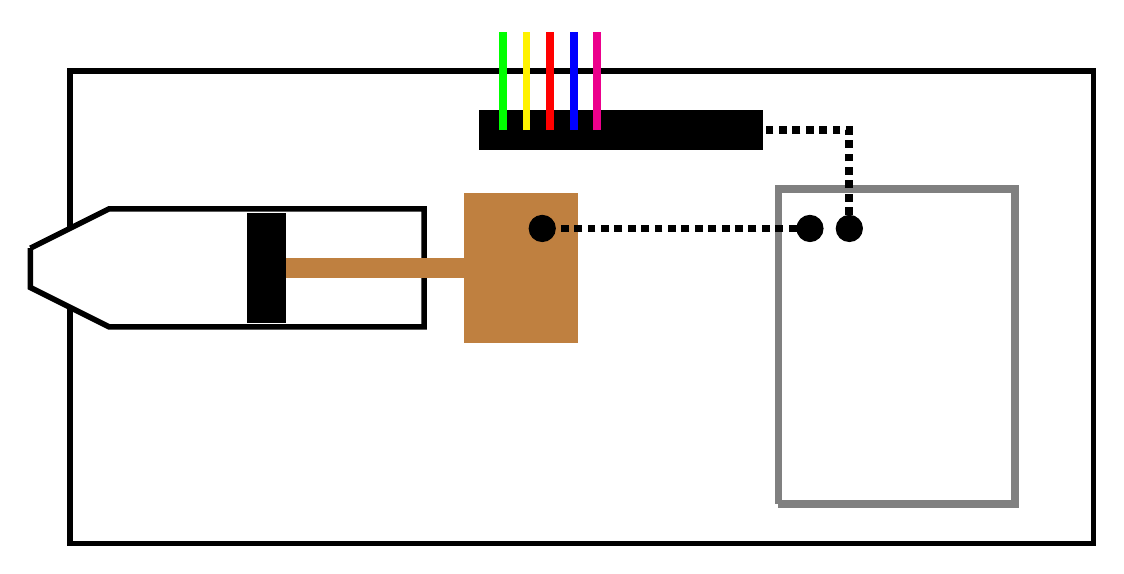
\begin{tikzpicture}
	% Hülle
	\draw[
		line width=0.07cm
	] (1,5) -- (1,2) -- (14,2) -- (14,8) -- (1,8) -- (1,6);
	% Spritze(oben)
	\draw[
		line width=0.07cm
	] (0.5,5.75) -- (0.5,5.25) -- (1.5,4.75) -- (5.5,4.75) -- (5.5,6.25) --
		(1.5,6.25) -- (0.5,5.75);
	% Arduino
	\draw[
		line width=0.1cm,
		color=gray
	] (10,2.5) -- (13,2.5) -- (13,6.5) -- (10,6.5) -- (10,2.5);
	% Servo(oben)
	\draw[
		line width=0.9cm,
		color=brown,
		fill=brown
	] (6,5) -- (7,5) -- (7,6) -- (6,6);
	% Kolben(oben)
	\draw[
		line width=0.5cm,
		color=black
	] (3.5,4.8) -- (3.5,6.2);
	% Verbindung Servo Kolben (oben)
	\draw[
		line width=0.25cm,
		color=brown
	] (3.75,5.5) -- (6,5.5);
	% Ansteuerung Servo (oben)
	\node[
		circle,
		draw,
		fill=black
	] at (10.4,6) {};
	\node[
		circle,
		draw,
		fill=black
	] at (7,6) {};
	\draw[
		dotted,
		color=black,
		line width=0.1cm
	] (10.4,6) -- (7,6);
	% Sensoren-Bank
	\draw[
		fill=black
	] (6.2,7) -- (9.8,7) -- (9.8,7.5) -- (6.2,7.5);
	% Sensoren
	\draw[
		color=green,
		line width=0.1cm
	] (6.5,7.25) -- (6.5,8.5);
	\draw[
		color=yellow,
		line width=0.1cm
	] (6.8,7.25) -- (6.8,8.5);
	\draw[
		color=red,
		line width=0.1cm
	] (7.1,7.25) -- (7.1,8.5);
	\draw[
		color=blue,
		line width=0.1cm
	] (7.4,7.25) -- (7.4,8.5);
	\draw[
		color=magenta,
		line width=0.1cm
	] (7.7,7.25) -- (7.7,8.5);
	% Sensoren Ansteuerung
	\node[
		circle,
		fill=black,
		draw
	] at (10.9,6) {};
	\draw[
		dotted,
		color=black,
		line width=0.1cm
	] (10.9,6) -- (10.9,7.25) -- (9.7,7.25);

\end{tikzpicture}
}
				\end{minipage}
				\begin{minipage}{\textwidth}
					\vspace{1cm}
					\begin{itemize}
						\item countersink nut into plunge
						\item translate rotation of threaded rod to lifting motion
						\item[$\Rightarrow$] compact design
					\end{itemize}
				\end{minipage}
			\end{column}
			\begin{column}{0.5\textwidth}
				\begin{center}
					\resizebox{0.5\textwidth}{!}{\includegraphics{pic/first-divetank}}
				\end{center}
			\end{column}
		\end{columns}
	\end{frame}
\end{document}
